\section{公式}

\begin{frame}[fragile]
\frametitle{数学模式}
\begin{itemize}
  \item<+-> 一切数学公式都要在数学模式下输入

    \begin{itemize}
      \item 不受外界字体命令控制
      \item 数学模式中空格不起作用,尽管用
      \item \alert{不建议用 MathType 生成 \LaTeX{} 公式}
      \item 建议始终调用 \pkg{amsmath} 宏包
    \end{itemize}

  \item<+-> 行内\zhparen{inline}公式

    \begin{itemize}
      \item 用一对美元符号(公式值千金):|$...$|
      \item 示例:理想气体状态方程可以写为 $PV=nRT$, 其中 $P$、$V$ 和 $T$
        分别是压强、体积和绝对温度
    \end{itemize}

  \item<+-> 独显\zhparen{display}公式

    \begin{itemize}
      \item 无编号:|\[...\]| 或 |equation*| 环境
      \item 编号:|equation| 环境
      \item \alert{不要用 \texttt{\$\$...\$\$}}
    \end{itemize}
\end{itemize}
\end{frame}

\begin{frame}[fragile]
\frametitle{结构}
\begin{itemize}
  \item 上下标

    \begin{itemize}
      \item |^| 和 |_|:|f^ab| 和 |f^{ab}|,|e^x^2|、|{e^x}^2| 和 |e^{x^2}|
      \item 张量:|R^a{}_b{}^{cd}| 或使用 \pkg{tensor} 宏包
      \item 配合积分、求和、极限使用:|\int|、|\sum|、|\lim|;
        \lstinline[style=style@inline]|\(no)limits|
    \end{itemize}

  \item 分式

    \begin{itemize}
      \item |\frac{〈分子〉}{〈分母〉}|
      \item 行内分式、小分式不好看:改用 |a/b|,或改用独显公式
      \item \alert{不推荐 \texttt{\textbackslash dfrac}}
    \end{itemize}

  \item 根式

    \begin{itemize}
      \item |\sqrt[〈次数〉]{〈内容〉}|
      \item 复杂情况改用分数指数:|{...}^{1/n}|
    \end{itemize}

  \item 矩阵与行列式

    \begin{itemize}
      \item |matrix|、|pmatrix|、|vmatrix| 等环境
      \item 语法类似表格:|&| 分列,|\\| 换行
      \item 推荐 \pkg{physics} 宏包
    \end{itemize}
\end{itemize}
\end{frame}

\begin{frame}[fragile]
\frametitle{括号与定界符}
\begin{itemize}
  \item<+-> 基本括号

    \begin{itemize}
      \item |(...)|、|[...]|、|\{...\}|、
      \item 绝对值、范数:\lstinline[style=style@inline]+|...|+ 或 |\vert...\vert|、|\Vert...\Vert|
      \item Dirac 符号:|\angle...\rangle|、\lstinline[style=style@inline]+|...\rangle+
    \end{itemize}

  \item<+-> 自动调节

    \begin{itemize}
      \item |\left(...\right)| 等
      \item 大型括号是拼出来的
    \end{itemize}

  \item<+-> 手动调节

    \begin{itemize}
      \item 只有 4 + 1 档:|\big|、|\Big|、|\bigg|、|\Bigg|
      \item 声明左中右:|\bigl|、|\bigm|、|\bigr| 等
    \end{itemize}
\end{itemize}
\end{frame}

\begin{frame}{符号与字体}
\begin{itemize}
  \item 符号不是按钮点出来的,也不是天上掉下来的 \pause

    \begin{itemize}
      \item (几乎)所有的符号都由字体提供 \pause
      \item 分清「它是什么」和「它长什么样」(术语:character 和 glyph)
    \end{itemize} \pause

  \item 寻找符号

    \begin{itemize}
      \item S. Pakin. \emph{The Comprehensive \LaTeX{} Symbol List}
            \link{https://ctan.org/pkg/comprehensive}
      \item 手写识别(不全):Detexify \link{http://detexify.kirelabs.org}
    \end{itemize} \pause

  \item 数学字体

    \begin{itemize}
      \item 你们要的「Times New Roman」:\pkg{newtxmath} 宏包
      \item \alert{不要用 \pkg{times} 和 \pkg{mathptmx} 宏包}
      \item 加粗:使用 \pkg{bm} 宏包
    \end{itemize} \pause

  \item 新方案:\pkg{unicode-math}

    \begin{itemize}
      \item 符号、字体、样式精调的一揽子解决方案
      \item 彻底修改底层,不可与传统方案混用
    \end{itemize}
\end{itemize}
\end{frame}

\begin{frame}[fragile]
\frametitle{多行公式}
\begin{itemize}
  \item 以下均要求 \pkg{amsmath} 宏包
  \item 独立数学环境

  \begin{itemize}
    \item 多行居中 |gather|、多行手动对齐 |align|、跨行 |multiline|
    \item 手动对齐:关系符前加 |&|
  \end{itemize}

  \item 内联数学环境

  \begin{itemize}
    \item 条件 |cases|、多行对齐 |split|、|...ed|
  \end{itemize} \pause

  \item 精细调整

  \begin{itemize}
    \item \pkg{mathtools}、\pkg{empheq} 等
    \item 自动换行:\pkg{breqn}
    \item \alert{避免使用 \texttt{eqnarray} 环境}
  \end{itemize}
\end{itemize}
\end{frame}

\begin{frame}[fragile]
\frametitle{专业功能(一)}
\begin{itemize}
  \item 更高更妙的物理:\pkg{physics} 宏包

    \begin{itemize}
      \item 括号:|\qty(...)|、|\qty\big{...}|
      \item 矩阵:|\mqty(...)|、\lstinline[style=style@inline]+\mqty|...|+|、\dmat{a,b,c,...}|
      \item Dirac 符号:|\ket|、|\bra|、|\ev|
      \item 向量、导数、微分、更多函数名……
    \end{itemize} \pause

  \item 国际单位:\pkg{siunitx} 宏包

    \begin{itemize}
      \item |$4.18 \times 10^3 J mol^{-1} K^{-1}$|

        \begin{itemize}
          \item $4.18 \times 10^3 J mol^{-1} K^{-1}$---No!
        \end{itemize}

      \item |\SI{4.18e3}{J.mol^{-1}.K^{-1}}|

        \begin{itemize}
          \item \SI{4.18e3}{J.mol^{-1}.K^{-1}}---Yes!
        \end{itemize} \pause

      \item 注 1:此宏包代码比 \LaTeX{} 内核还长 \pause
      \item 注 2:新定义并不会影响使用
            \link{https://en.wikipedia.org/wiki/2019_redefinition_of_SI_base_units}
    \end{itemize}
\end{itemize}
\end{frame}

\begin{frame}{专业功能(二)}
\begin{columns}
\begin{column}{0.65\textwidth}
  \begin{itemize}
    \item 花式图表

      \begin{itemize}
        \item Feynman 图:\pkg{tikz-feynman} 宏包%
              \zhparen{arXiv: 1601.05437 \link{https://arxiv.org/abs/1601.05437}}
        \item Feynman 斜线:\pkg{slashed} 宏包
        \item Wick 定理:\pkg{simplewick} 宏包、\pkg{simpler-wick} 宏包
        \item Young 表、Young 图:\pkg{ytableau} 宏包
        \item 电路图:\pkg{circuitikz} 宏包
        \item 拓扑量子场论:\pkg{tqft} 宏包
        \item ……
      \end{itemize}
  \end{itemize}
\end{column} \pause
\begin{column}{0.3\textwidth}
  \hspace{-0.15\textwidth}
  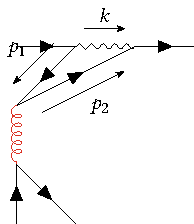
\includegraphics[width=\textwidth]{example/feynman-diag.pdf}
\end{column}
\end{columns}
\end{frame}

\begin{frame}[fragile]
\frametitle{专业功能(三)}
\begin{itemize}
  \item 抄录:忽略所有特殊类别码\zhparen{catcode},原样显示

    \begin{itemize}
      \item |\verb〈char〉...〈char〉|、|verbatim| 环境
      \item \pkg{verbatim}、\pkg{fancyvrb} 宏包
    \end{itemize} \pause

  \item 语法高亮

    \begin{itemize}
      \item \pkg{listings} 宏包
      \item \pkg{minted} 宏包

        \begin{itemize}
          \item 需要 Python,且开启 |--shell-escape|
        \end{itemize}
    \end{itemize}
\end{itemize} \pause
\begin{lstlisting}[
  language         = C,
  basewidth        = 0.54em,
  xleftmargin      = 6em,
  numbers          = left,
  numberstyle      = \tiny,
  basicstyle       = \scriptsize\ttfamily,
  keywordstyle     = \color{emph1},
  commentstyle     = \itshape\color{comment},
  stringstyle      = \color{texcs},
  showstringspaces = false]
/* A standard Hello World program in C. */
#include <stdio.h>

int main(int argc, char** argv) {
    printf("Hello, world!\n");
    return 0;
}
\end{lstlisting}
\vspace{-1cm}
\end{frame}
